\documentclass[11pt]{article}
\title{Meccano triangles}
\author{https://github.com/heptagons/meccano/nest}
\date{}

\newfam\bbbfam
\font\bbbten=msbm10
\font\bbbseven=msbm7
\font\bbbfive=msbm5
\textfont\bbbfam=\bbbten
\scriptfont\bbbfam=\bbbseven
\scriptscriptfont\bbbfam=\bbbfive
\def\bbb{\fam=\bbbfam}

\usepackage{../../meccano}
\begin{document}

\maketitle
\begin{abstract}
We construct meccano triangles. Basic triangles has the three sides as integers and calculate the internal diagonal distances.
Such diagonals then are used as the new side of more complicated triangles and then again we
calculate new distances formed and so on. Eventually we expect to
find certain angles joining the triangles which can be used to construct regular polygons or more figures.
\end{abstract}

\section{Basic triangle}
A basic triangle has the tree sides $a$, $b$ and $c$ where $a,b,c \in \bbb N$. To avoid repetitions we
consider only the cases $a \ge b$, $b \ge c$ and $a \ge c$. Valid triangles also need the 
condition $b + c > a$.

\subsection{Basic triangle diagonals}

To calculate the diagonals from side $a$ to side $b$ we start calculating $\cos{C}$ where $C$ is the
opposite angle of side $c$:
\begin{align}
\cos{C} &= \frac{a^2 + b^2 - c^2}{2ab}
\end{align}

Then with the $\cos{C}$ we can calculate every diagonal $\overline{a_xb_y}$ with
the law of cosines:
\begin{align}
\overline{a_xb_y} &= \sqrt{x^2 + y^2 - 2xy\cos{C}}\\
       &= \sqrt{x^2 + y^2 - 2xy\frac{a^2 + b^2 - c^2}{2ab}}\\
       &= \frac{\sqrt{a^2b^2(x^2 + y^2)-abxy(a^2 + b^2 - c^2)}}{ab}
\end{align}

where $1 \le x \le a$, $1 \le y \le b$ and $x - y \ge 0$.

By inspection we deduce that for basic meccano triangles:
\begin{align}
a, b, c &\in \bbb{N}\\
\cos{A}, \cos{B}, \cos{C} &\in \bbb{Q}\\
\overline{a_xb_y}, \overline{b_yc_z}, \overline{a_xc_z} &\in \bbb{A}
\end{align}

\subsection{Example triangle [7,6,5]}

\begin{figure}[htp]
\centering
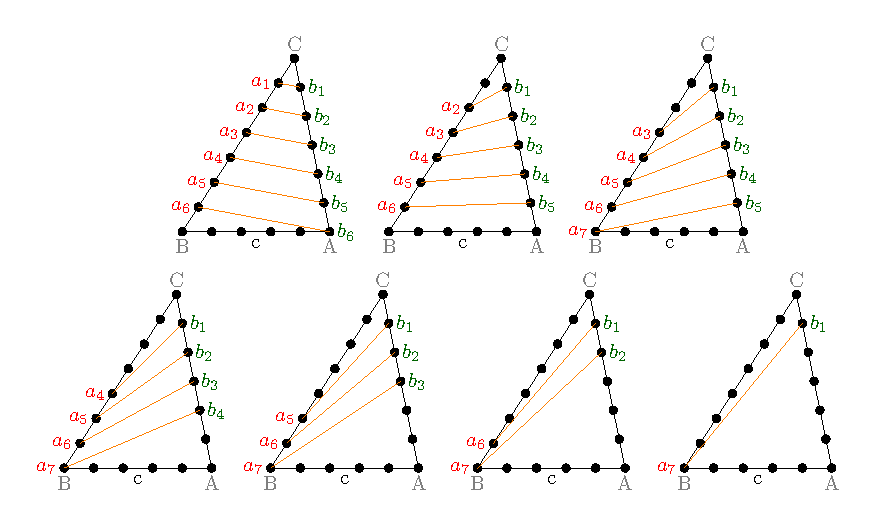
\includegraphics[scale=1]{t765ab}
\caption{Triangle $[7,6,5]$, $a_xb_x$ diagonals.}
\label{t765ab}
\end{figure}

Figure \ref{t765ab} show triangle $[7,6,5]$ diagonals $a_xb_y$.
The diagonals join points from side $a$ nodes described as $a_x$ to side $b$ nodes described as $b_y$ in all combinations.
Next matrix show the diagonals values:
\[
a_xb_y = \begin{bmatrix}
	\frac{2\sqrt7}7 & \frac{\sqrt{105}}7 & \frac{2\sqrt{70}}7 & \frac{\sqrt{553}}7 & \frac{2\sqrt{231}}7 & \frac{\sqrt{1393}}7 & 2\sqrt{10} \\
	 & \frac{4\sqrt7}7 & \frac{\sqrt{217}}7 & \frac{2\sqrt{105}}7 & \frac{\sqrt{721}}7 & \frac{4\sqrt{70}}7 & \sqrt{33} \\
	 & & \frac{6\sqrt7}7 & \frac{\sqrt{385}}7 & \frac{2\sqrt{154}}7 & \frac{3\sqrt{105}}7 & 2\sqrt{7} \\
	 & & & \frac{8\sqrt7}7 & \frac{\sqrt{609}}7 & \frac{2\sqrt{217}}7 & 5 \\
	 & & & & \frac{10\sqrt7}7 & \frac{\sqrt{889}}7 & 2\sqrt{6} \\
	 & & & & & \frac{12\sqrt7}7 \\
\end{bmatrix}
\]

\begin{figure}[htp]
\centering
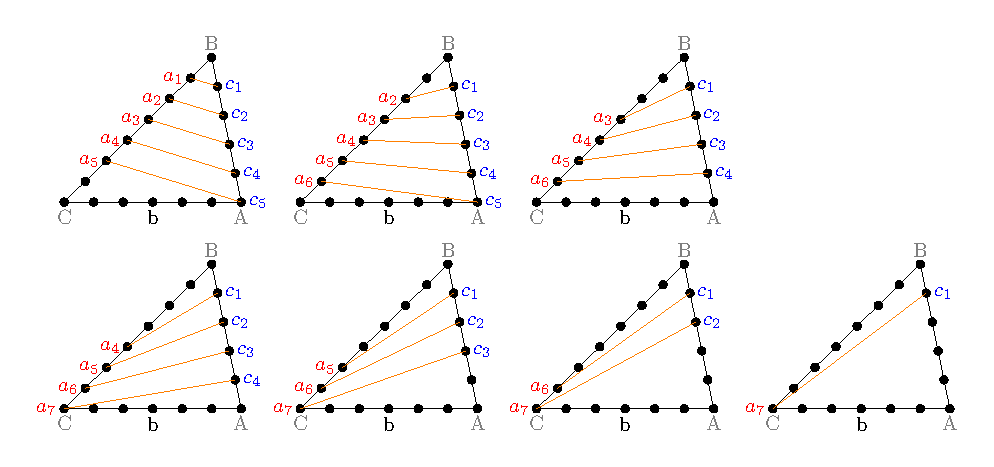
\includegraphics[scale=1]{t765ac}
\caption{Triangle $[7,6,5]$, $a_xc_z$ diagonals.}
\label{t765ac}
\end{figure}

Figure \ref{t765ac} show triangle $[7,6,5]$ diagonals $a_xc_z$.
The diagonals join points from side $a$ nodes described as $a_x$ to side $c$ nodes described as $c_z$ in all combinations.
Next matrix show the diagonals values:
\[
a_xc_z = \begin{bmatrix}
	\frac{4\sqrt{70}}{35} & \frac{3\sqrt{385}}{35} \\
	& \frac{8\sqrt{70}}{35} & \frac{\sqrt{7945}}{35} \\
	& & \frac{12\sqrt{70}}{35} & \frac{\sqrt{14665}}{35} \\
	& & & \frac{16\sqrt{70}}{35} & \frac{3\sqrt{105}}{7} \\
	& & & & \frac{4\sqrt{70}}{7} & \frac{\sqrt{1393}}{7} \\
\end{bmatrix}
\]

\end{document}